% =====================================================================
%  Review-II Report -- Final Year Project
%  Compile with pdfLaTeX (twice, so the contents/figure lists resolve).
%  Overleaf: upload this folder (r2_reviewreport.tex, ssnreview.cls,
%  ssn-logo.png, figures/) and set the main document to this file.
%
%  Every number in this report is taken from the project repository
%  (audit/, derivatives/, docs/). Figures in figures/ are regenerated by
%  scripts/report/make_review2_figures.py.
%
%  Items shown in red (\todo{...}) must be filled in before submission.
% =====================================================================
\PassOptionsToPackage{obeyspaces,spaces}{url}
\PassOptionsToPackage{table}{xcolor}
\documentclass{ssnreview}

% ---- extra packages (all available on Overleaf / TeX Live) ----------
\usepackage{amsmath,amssymb}
\usetikzlibrary{positioning,arrows.meta,calc}
\setlength{\emergencystretch}{3em}  % avoid overfull lines caused by long file names
\usepackage[most]{tcolorbox}

% ---- colours and styling (match the presentation theme) --------------
\definecolor{SSNBlue}{RGB}{16,62,110}
\definecolor{AccentBlue}{RGB}{30,136,229}
\definecolor{LightBlue}{RGB}{232,242,252}
\definecolor{DoneGreen}{RGB}{27,122,61}
\definecolor{PlanOrange}{RGB}{194,98,0}
\newcommand{\hdr}{\rowcolor{SSNBlue!12}}                      % table header row
\newcommand{\statusdone}{\textcolor{DoneGreen}{\textbf{Completed}}}
\newcommand{\statusplan}{\textcolor{PlanOrange}{\textbf{Planned}}}
\setlength{\aboverulesep}{0pt}
\setlength{\belowrulesep}{0pt}
\newtcolorbox{keybox}[1]{enhanced, breakable, colback=LightBlue,
  colframe=SSNBlue, coltitle=white, fonttitle=\bfseries, title=#1,
  arc=2pt, boxrule=0.6pt, left=6pt, right=6pt, top=4pt, bottom=4pt,
  before skip=10pt, after skip=10pt}
\newtcolorbox{modulebox}{enhanced, breakable, colback=LightBlue!45,
  colframe=SSNBlue!55, arc=2pt, boxrule=0.5pt, left=4pt, right=6pt,
  top=2pt, bottom=2pt}

\newcommand{\todo}[1]{\textcolor{red}{[#1]}}
\DeclareUrlCommand\code{\urlstyle{tt}}  % breakable typewriter text for paths/identifiers
\renewcommand{\arraystretch}{1.3}

% ---- title-page metadata --------------------------------------------
\projecttitle{Assessment of Alzheimer's Disease Progression Using a\\
Comorbidity-Aware Meta-Bayesian Framework with\\ Resting-State fMRI}
\reviewnumber{REVIEW REPORT -- II}
\students{%
  Harishkanna R \todo{Register No.}\\
  \todo{Student Name 2 (Register No.)}\\
  \todo{Student Name 3 (Register No.)}}
\supervisor{\todo{Dr./Mr./Ms. Supervisor Name}}
\department{Department of Computer Science and Engineering}
\institution{Sri Sivasubramaniya Nadar College of Engineering}
\academicyear{2026--2027}
\collegelogo{ssn-logo.png}

\begin{document}
\makereviewtitle
\reviewfrontmatter

% =====================================================================
\begin{reviewabstract}
Alzheimer's disease (AD) develops over many years, moving from cognitively
normal ageing through subjective memory complaints and successive stages of
mild cognitive impairment (MCI) before dementia. Detecting where a person sits
on this continuum, rather than only separating AD from healthy controls, is
what makes early intervention possible. This project stages AD progression
across six ordered classes (CN $\rightarrow$ SMC $\rightarrow$ EMCI
$\rightarrow$ MCI $\rightarrow$ LMCI $\rightarrow$ AD) from resting-state
functional MRI (rs-fMRI) of the Alzheimer's Disease Neuroimaging Initiative
(ADNI). The planned model combines a multi-attention transformer, meta-learning
and comorbidity fusion with a Bayesian ordinal classifier that reports
uncertainty with each prediction.

This report covers the data foundation built since the first review. The ADNI
data has no T1-weighted anatomical image and no recoverable slice-timing
metadata, so every processing step was designed around a BOLD-only dataset.
175 acquisitions were audited and 29 missing scans were recovered from raw
DICOM. Two acquisitions were excluded with documented reasons. A
fixed pipeline was then applied: motion correction, direct EPI-to-MNI
registration, nuisance regression and band-pass filtering. It produced 165
preprocessed scans from 127 subjects. The 8 remaining scans were rejected
because their TR of 6.02~s makes the 0.01--0.10~Hz band invalid. Each scan was
parcellated with the Brainnetome-246 atlas into ALFF, ReHo, functional
connectivity (FC) and degree-centrality (DC) biomarkers. These were then
normalised within each subject, so no information leaks across subjects. All 165
scans passed the independent consistency checks. Recomputing DC from the stored FC
matrices matched exactly (difference $0.0$). The dataset-scale code reproduced the
validated pilot bit for bit. One nominal feature, FC strength, turned out to be
exactly DC/245 and was removed. Each scan is therefore described by a
$246\times3$ regional matrix and a $246\times246$ Fisher-$z$ connectivity matrix.
The modelling stages are specified and scheduled. Their evaluation will use
subject-grouped, stratified cross-validation.

\keywords{Alzheimer's disease; resting-state fMRI; ADNI; Brainnetome atlas;
ALFF; ReHo; functional connectivity; ordinal classification; Bayesian deep
learning; meta-learning}
\end{reviewabstract}

\chapter*{List of Abbreviations}
\addcontentsline{toc}{chapter}{List of Abbreviations}
\begin{table}[H]
\centering
\small
\begin{tabular}{>{\bfseries}l@{\hspace{1.2cm}}l}
\toprule
\hdr Abbreviation & Expansion\\
\midrule
AD & Alzheimer's disease\\
ADNI & Alzheimer's Disease Neuroimaging Initiative\\
ALFF & Amplitude of low-frequency fluctuation\\
BIDS & Brain Imaging Data Structure\\
BOLD & Blood-oxygen-level-dependent\\
CN & Cognitively normal\\
CSF & Cerebrospinal fluid\\
CV & Cross-validation\\
DC & Degree centrality\\
DVARS & Temporal derivative RMS variance\\
EMCI & Early mild cognitive impairment\\
EPI & Echo-planar imaging\\
FC & Functional connectivity\\
FCS & FC strength\\
FD & Framewise displacement\\
FWHM & Full width at half maximum\\
LMCI & Late mild cognitive impairment\\
MCI & Mild cognitive impairment\\
MNI & Montreal Neurological Institute\\
QC & Quality control\\
ReHo & Regional homogeneity\\
ROI & Region of interest\\
rs-fMRI & Resting-state functional MRI\\
SMC & Subjective memory concern\\
SNR & Signal-to-noise ratio\\
TR & Repetition time\\
tSNR & Temporal signal-to-noise ratio\\
WM & White matter\\
\bottomrule
\end{tabular}
\end{table}

% =====================================================================
\chapter{Introduction}

Alzheimer's disease is the most common cause of dementia and is a growing
burden on ageing populations~\cite{alz2024,livingston2020}. Its pathology starts
years before clinical symptoms appear. It is now viewed as a continuum: from
cognitively normal (CN) ageing, to subjective cognitive decline or subjective
memory concern (SMC)~\cite{jessen2014}, to early, intermediate and late mild
cognitive impairment (EMCI, MCI, LMCI)~\cite{petersen2010}, and finally to
dementia due to AD. Intervention is most promising in the early stages. So the
clinically useful question is not only ``does this person have AD?'' but
``where on the continuum is this person?''

Resting-state functional MRI (rs-fMRI) measures spontaneous low-frequency
fluctuations of the blood-oxygen-level-dependent (BOLD) signal while the subject
lies at rest~\cite{biswal1995}. It needs no task performance, which makes it
practical for cognitively impaired patients. AD-related disruption of
intrinsic networks, notably the default-mode network, was reported early on~\cite{greicius2004}.
Regional measures such as the amplitude of low-frequency fluctuation
(ALFF)~\cite{zang2007} and regional homogeneity (ReHo)~\cite{zang2004}, together
with network measures such as functional connectivity (FC) and degree
centrality (DC)~\cite{zuo2012}, capture complementary aspects of this
disruption.

Imaging alone ignores factors that change an individual's risk and
trajectory. Examples are age, sex, cognitive status and vascular or metabolic
comorbidities~\cite{livingston2020}. AD stages are
also \emph{ordered}: confusing CN with SMC is a smaller error than confusing CN
with AD. Treating staging as flat multi-class classification ignores this
structure. These two observations motivate the project. It aims to build a
\emph{comorbidity-aware}, \emph{ordinal} and \emph{uncertainty-reporting}
staging model on top of a carefully validated rs-fMRI feature set.

\section{Scope of this Review}
The first review fixed the problem, the six-class progression ordering and the
overall architecture. Since then the work has concentrated on the data
foundation that every later stage depends on. That covers dataset audit and recovery,
preprocessing of all six groups, quality control (QC), Brainnetome-246
parcellation, biomarker generation, independent validation and leakage-free
within-subject normalisation. All of these are complete for the full dataset
and are reported here with their verification evidence. The learning stages
(multi-attention transformer, meta-learning, comorbidity fusion and Bayesian
ordinal classifier) are specified in Chapter~\ref{ch:methodology}. They are scheduled in
Section~\ref{sec:plan} but are not yet implemented, and no model
results are claimed in this report.

\begin{table}[H]
\centering
\caption{Project progress at a glance}\label{tab:status}
\small
\begin{tabularx}{\textwidth}{>{\raggedright\arraybackslash}p{5.2cm}>{\centering\arraybackslash}p{2.2cm}X}
\toprule
Stage & Status & Evidence\\
\midrule
Dataset audit, DICOM recovery, exclusions & \statusdone & 175 audited, 29 recovered, 2 excluded\\
Slice-timing investigation & \statusdone & not recoverable; not performed\\
Preprocessing and QC (6 groups) & \statusdone & 165 of 173 eligible scans\\
Brainnetome-246 parcellation & \statusdone & 246/246 ROIs in 165/165 scans\\
ALFF, ReHo, FC, DC biomarkers & \statusdone & 165/165 pass independent checks\\
Within-subject normalisation & \statusdone & 165/165, 0 failures\\
Comorbidity data cleaning & \statusplan & LMCI tables missing\\
Grouped CV folds, train-fold scaling & \statusplan & --\\
Multi-attention transformer & \statusplan & --\\
Meta-learning, comorbidity fusion & \statusplan & --\\
Bayesian ordinal classifier, uncertainty, XAI & \statusplan & --\\
\bottomrule
\end{tabularx}
\end{table}

\begin{keybox}{Highlights of this review}
\begin{itemize}[leftmargin=*, itemsep=1pt]
  \item \textbf{165} preprocessed rs-fMRI scans from \textbf{127} subjects
        across six stages, every exclusion documented.
  \item \textbf{246/246} Brainnetome regions covered in every scan.
  \item DC recomputed from stored FC matches \textbf{exactly} (difference
        0.0) in all 165 scans; the dataset code reproduces the validated
        pilot \textbf{bit for bit}.
  \item Model-ready features per scan: $\mathbf{246\times3}$ regional
        (mALFF, mReHo, DC$_z$) $+$ $\mathbf{246\times246}$ Fisher-$z$ FC.
  \item No metadata was guessed: slice timing, tissue maps and invalid
        filter bands are handled by documented exclusion or substitution.
\end{itemize}
\end{keybox}

\section{Objectives}
\begin{enumerate}[label=\arabic*.]
  \item To curate an analysis-ready ADNI rs-fMRI cohort covering six diagnostic
        stages, with every exclusion, recovery and metadata limitation
        documented rather than assumed.
  \item To design and implement a reproducible, BOLD-only preprocessing
        pipeline with per-acquisition quality control and full provenance.
  \item To extract regional (ALFF, ReHo, DC) and network (FC) biomarkers on the
        Brainnetome-246 atlas and to verify them independently of the code
        that generated them.
  \item To build a leakage-free, model-ready feature representation for every
        acquisition.
  \item To develop a comorbidity-aware Meta-Bayesian model, combining a
        multi-attention transformer, meta-learning, comorbidity fusion and a
        Bayesian ordinal classifier, that stages AD progression with calibrated
        uncertainty.
  \item To evaluate the model under subject-grouped cross-validation with
        ordinal and calibration metrics, and to explain its predictions at the
        level of brain regions.
\end{enumerate}
Objectives 1--4 are complete; objectives 5--6 form the remaining work.

\section{Organisation of the Report}
Chapter~\ref{ch:queries} answers the queries raised in the first review.
Chapter~\ref{ch:problem} states the problem formally. Chapter~\ref{ch:methodology}
presents the architecture and modules. Chapter~\ref{ch:implementation}
describes the implementation, and Chapter~\ref{ch:results} reports and discusses
the results obtained so far, together with the limitations and the plan for
the remaining work.

% =====================================================================
\chapter{First Review -- Queries and Answers}\label{ch:queries}

% TODO: replace the placeholders below with the exact queries raised by the
% Review-I panel and the corresponding answers.
\begin{itemize}
  \item \textbf{Query 1:} \todo{Query raised by the panel in Review I.}\\
        \textbf{Answer:} \todo{Answer and the section of this report where it
        is addressed.}
  \item \textbf{Query 2:} \todo{Query raised by the panel in Review I.}\\
        \textbf{Answer:} \todo{Answer.}
  \item \textbf{Query 3:} \todo{Query raised by the panel in Review I.}\\
        \textbf{Answer:} \todo{Answer.}
\end{itemize}

\section{Design Revisions Since Review I}
Verifying the data turned up several facts that change or tighten the Review-I
design. They are listed here so that the panel can see what changed and why.

\begin{enumerate}[label=\textbf{R\arabic*.}]
  \item \textbf{Regional feature matrix is $246\times3$, not $246\times4$.}
        The Review-I design used four regional biomarkers (ALFF, ReHo, DC, FC
        strength). FC strength is the \emph{mean} of a region's off-diagonal
        connectivity and DC is the \emph{sum} of the same entries, so
        $\text{FCS}_i = \text{DC}_i/245$ exactly (measured Pearson
        $r = 1.0$; maximum deviation $6.9\times10^{-18}$ over 40,590 region
        values). FC strength carries no independent information and was
        removed from the feature set (Section~\ref{sec:impl-norm}).
  \item \textbf{Effective sample size is 127 subjects, not 165 scans.}
        96 subjects have one scan, 25 have two, 5 have three and 1 has four.
        MCI is the largest class by scans (32) but the smallest by subjects
        (14). All validation splits will therefore be grouped by subject
        (Section~\ref{sec:m6}).
  \item \textbf{No AD acquisition is unrecoverable.} An earlier working note
        listed 6 of 25 AD scans as unrecoverable. A re-audit located all 6 as
        valid, checksummed NIfTI files, and all 25 AD scans were processed.
  \item \textbf{Progression ordering is held fixed} as
        CN $\rightarrow$ SMC $\rightarrow$ EMCI $\rightarrow$ MCI $\rightarrow$
        LMCI $\rightarrow$ AD. The ordinal loss depends on it.
  \item \textbf{Hypertension and diabetes are not directly available.} The
        supplied ADNI medical-history tables carry only broad categories
        (cardiovascular, endocrine-metabolic). The comorbidity module will use
        these categories under their real names instead of relabelling them
        as specific diseases.
\end{enumerate}

% =====================================================================
\chapter{Problem Statement}\label{ch:problem}

\paragraph{Task.} Given the resting-state fMRI acquisition(s) and the clinical
and comorbidity record of a subject, estimate the subject's stage on the
ordered scale
\[
  y \in \{0{:}\,\text{CN},\ 1{:}\,\text{SMC},\ 2{:}\,\text{EMCI},\
  3{:}\,\text{MCI},\ 4{:}\,\text{LMCI},\ 5{:}\,\text{AD}\},
\]
and report a predictive distribution $p(y \mid \mathbf{X}, \mathbf{c})$ whose
spread reflects the model's uncertainty.

\paragraph{Inputs.}
\begin{itemize}
  \item A 4-D BOLD time series per acquisition (ADNI, Philips scanners,
        mostly TR $\approx 3.0$~s, 140 volumes, $\approx 3.3$~mm voxels).
  \item From it, after this review's work: a regional feature matrix
        $\mathbf{R} \in \mathbb{R}^{246\times3}$ (mALFF, mReHo, DC$_z$) and a
        connectivity matrix $\mathbf{Z} \in \mathbb{R}^{246\times246}$
        (Fisher-$z$ FC).
  \item A comorbidity vector $\mathbf{c}$: age, sex, and clinical and
        medical-history variables where available.
\end{itemize}

\paragraph{Outputs.} A stage estimate $\hat{y}$, the full distribution
$p(y\mid\cdot)$, an uncertainty measure, and region-level explanations.

\paragraph{Constraints.}
\begin{itemize}
  \item \textbf{BOLD-only data:} no T1-weighted image for any subject, so no
        anatomical registration or tissue segmentation is possible.
  \item \textbf{No slice-timing metadata} in any of the 175 JSON sidecars or
        in the raw DICOM headers. Nothing may be inferred or fabricated.
  \item \textbf{Heterogeneous TR:} most scans use TR $\approx 3.0$~s, one uses
        2.25~s and eight use $\approx 6.02$~s. The last group is incompatible
        with the fixed 0.01--0.10~Hz band.
  \item \textbf{Small, imbalanced cohort:} 127 subjects, with as few as 14 in
        one class. One group (LMCI) has no clinical cohort table yet.
  \item \textbf{Compute:} a single workstation under WSL2. Processing is
        restricted to one worker and one acquisition at a time.
\end{itemize}

\paragraph{Success criteria.}
\begin{itemize}
  \item \textbf{Data level (this review):} every acquisition accounted for,
        with no fabricated metadata, no NaN/Inf values, and biomarkers that
        agree exactly with their documented definitions when recomputed.
  \item \textbf{Model level (final review):} under repeated, stratified,
        subject-grouped cross-validation, report balanced accuracy, mean
        absolute stage error, quadratic weighted Cohen's $\kappa$ and expected
        calibration error, compared with non-ordinal and non-comorbidity
        baselines.
\end{itemize}

% =====================================================================
\chapter{Methodology}\label{ch:methodology}

The workflow has two halves. The \emph{data foundation} (Modules~1--4) turns
raw ADNI acquisitions into validated, model-ready features. The
\emph{modelling} half (Module~5) learns the staging model. Module~6
(testing and evaluation) runs through both halves.

\section{Proposed Workflow}
\begin{enumerate}[label=\textbf{Step \arabic*:}]
  \item Audit the raw ADNI data, recover missing scans from DICOM, document
        exclusions and organise everything in a BIDS-style layout.
  \item Preprocess every eligible BOLD acquisition with a single frozen
        pipeline and compute per-acquisition QC.
  \item Align the Brainnetome-246 atlas to each acquisition and extract ROI
        time series, ALFF, ReHo, FC and DC.
  \item Validate every biomarker independently and normalise within subject.
  \item Build subject-level, stratified, grouped cross-validation folds and
        fit cross-subject scaling on training folds only.
  \item Train the multi-attention transformer with meta-learning, fuse
        comorbidity information, and stage with a Bayesian ordinal head.
  \item Evaluate with ordinal and calibration metrics, and explain predictions.
\end{enumerate}

\section{Architectural Design for Proposed System}

Figure~\ref{fig:architecture} shows the complete system. Solid blocks are
implemented and verified. Dashed blocks are the modelling stages still to
be implemented.

\begin{figure}[H]
\centering
\resizebox{\textwidth}{!}{%
\begin{tikzpicture}[
  node distance=0.45cm,
  >={Stealth[length=2.2mm]},
  blk/.style={draw, rounded corners, thick, align=center, font=\small,
              text width=4.4cm, minimum height=0.95cm,
              execute at begin node={\hyphenpenalty=10000\exhyphenpenalty=10000}},
  done/.style={blk, fill=green!8},
  data/.style={blk, fill=blue!8},
  plan/.style={blk, dashed, fill=orange!10},
  lbl/.style={font=\bfseries\small, align=center}]
  % column 1 -- data and preprocessing
  \node[data] (adni) {ADNI rs-fMRI\\ raw DICOM + partial NIfTI};
  \node[done, below=of adni] (audit) {Data audit, DICOM recovery, exclusions, BIDS layout};
  \node[done, below=of audit] (st) {Slice-timing investigation\\ (not recoverable)};
  \node[done, below=of st] (pre) {Preprocessing: motion correction, EPI$\rightarrow$MNI, 4\,mm resampling, 6\,mm FWHM, detrend, nuisance, 0.01--0.10\,Hz};
  \node[done, below=of pre] (qc) {Per-acquisition QC\\ tSNR, SNR, FD, DVARS, entropy};
  % column 2 -- features
  \node[done, right=0.7cm of adni] (bn) {Brainnetome-246 alignment\\ (nearest neighbour)};
  \node[done, below=of bn] (ts) {ROI time series\\ $135\times246$};
  \node[done, below=of ts] (bio) {ALFF $\cdot$ ReHo $\cdot$ FC $\cdot$ DC\\ + independent validation};
  \node[done, below=of bio] (norm) {Within-subject normalisation\\ $246\times3$ + $246\times246$};
  \node[data, below=of norm] (com) {Comorbidity data\\ age, sex, clinical scores, medical history};
  % column 3 -- modelling
  \node[plan, right=0.7cm of bn] (cv) {Subject-grouped CV folds\\ train-fold-only scaling};
  \node[plan, below=of cv] (mat) {Multi-Attention\\ Transformer};
  \node[plan, below=of mat] (meta) {Meta-learning\\ (episodic training)};
  \node[plan, below=of meta] (fuse) {Comorbidity fusion};
  \node[plan, below=of fuse] (ord) {Bayesian ordinal classifier\\ stage + uncertainty + XAI};
  % arrows
  \foreach \a/\b in {adni/audit, audit/st, st/pre, pre/qc, bn/ts, ts/bio, bio/norm,
                     cv/mat, mat/meta, meta/fuse, fuse/ord}
    \draw[->, thick] (\a) -- (\b);
  \draw[->, thick] (qc.east) -- ++(0.35,0) |- (bn.west);
  \draw[->, thick] (norm.east) -- ++(0.2,0) |- (cv.west);
  \draw[->, thick, dashed] (com.east) -- ++(0.48,0) |- (fuse.west);
  % column titles
  \node[lbl, above=0.25cm of adni] {Data \& preprocessing};
  \node[lbl, above=0.25cm of bn] {Feature extraction};
  \node[lbl, above=0.25cm of cv] {Modelling (planned)};
\end{tikzpicture}}
\caption{Architecture of the proposed system. Solid boxes: implemented and
verified for all 165 acquisitions. Dashed boxes: planned modelling stages.}
\label{fig:architecture}
\end{figure}

\section{Modules}
For each module the purpose, inputs, processing, outputs and dependencies are
given below. Implementation detail follows in Chapter~\ref{ch:implementation}.

\subsection{Module 1: Data Acquisition, Audit and Curation}
\begin{modulebox}\begin{description}[leftmargin=2.6cm, style=nextline, font=\normalfont\bfseries\color{SSNBlue}]
  \item[Purpose] Produce a complete, documented inventory of usable BOLD
        acquisitions before any processing time is spent.
  \item[Inputs] ADNI raw DICOM archives, pre-converted NIfTI files and JSON
        sidecars for six groups; ADNI image-collection and clinical tables.
  \item[Processing] Inventory audit; recovery of NIfTI-missing records from
        raw DICOM; duplicate/orphan/MD5 hash-collision audit; exclusion
        register; BIDS-style organisation with
        \code{participants.tsv} as the single source of group labels;
        slice-timing investigation over JSON and DICOM headers.
  \item[Outputs] 173 eligible acquisitions; \code{audit/excluded_runs.csv};
        audit reports under \code{audit/}.
  \item[Dependencies] dcm2niix (DICOM to NIfTI), Python (pandas, pydicom).
\end{description}\end{modulebox}

\subsection{Module 2: rs-fMRI Preprocessing}
\begin{modulebox}\begin{description}[leftmargin=2.6cm, style=nextline, font=\normalfont\bfseries\color{SSNBlue}]
  \item[Purpose] Remove non-neural signal and bring every scan into a common
        space, using one frozen pipeline for all groups.
  \item[Inputs] Eligible 4-D BOLD acquisitions.
  \item[Processing] Input validation $\rightarrow$ discard 5 volumes
        $\rightarrow$ motion correction $\rightarrow$ direct EPI-to-MNI
        registration $\rightarrow$ 4~mm resampling $\rightarrow$ 6~mm
        smoothing $\rightarrow$ linear detrending $\rightarrow$ nuisance
        regression $\rightarrow$ 0.01--0.10~Hz band-pass, followed by QC.
  \item[Outputs] Preprocessed BOLD ($46\times55\times46\times135$, 4~mm),
        brain mask, motion parameters, nuisance design matrix, provenance JSON
        and a QC folder per acquisition.
  \item[Dependencies] FreeSurfer 7.4.1 FS-FAST, ANTsPy, Nilearn, TemplateFlow,
        SciPy.
\end{description}\end{modulebox}

\subsection{Module 3: Parcellation and Biomarker Extraction}
\begin{modulebox}\begin{description}[leftmargin=2.6cm, style=nextline, font=\normalfont\bfseries\color{SSNBlue}]
  \item[Purpose] Summarise each scan as interpretable regional and network
        biomarkers on a fine-grained, connectivity-based atlas~\cite{fan2016}.
  \item[Inputs] Preprocessed BOLD, Brainnetome-246 atlas and look-up table.
  \item[Processing] Lossless atlas reorientation and nearest-neighbour
        alignment; ROI time series; voxel-wise ALFF and ReHo aggregated to
        ROIs; ROI-level FC and DC; independent recomputation checks.
  \item[Outputs] Per acquisition: ROI time series ($135\times246$), ALFF,
        ReHo, DC ($246$ each), FC ($246\times246$), QC and metadata.
  \item[Dependencies] Module 2; NumPy, SciPy, NiBabel, Nilearn.
\end{description}\end{modulebox}

\subsection{Module 4: Feature Normalisation and Model-Ready Representation}
\begin{modulebox}\begin{description}[leftmargin=2.6cm, style=nextline, font=\normalfont\bfseries\color{SSNBlue}]
  \item[Purpose] Remove scanner- and subject-specific scaling without
        letting any information cross between subjects.
  \item[Inputs] Raw biomarkers from Module 3.
  \item[Processing] Within-subject transforms (mALFF, mReHo, DC$_z$,
        Fisher-$z$ FC); redundancy analysis (FC strength removed).
  \item[Outputs] $\mathbf{R}\in\mathbb{R}^{246\times3}$ and
        $\mathbf{Z}\in\mathbb{R}^{246\times246}$ per acquisition, written to a
        separate output tree.
  \item[Dependencies] Module 3.
\end{description}\end{modulebox}

\subsection{Module 5: Comorbidity-Aware Meta-Bayesian Staging Model (planned)}
\begin{modulebox}\begin{description}[leftmargin=2.6cm, style=nextline, font=\normalfont\bfseries\color{SSNBlue}]
  \item[Purpose] Map imaging features and comorbidity information to an ordinal
        stage with calibrated uncertainty.
  \item[Inputs] $\mathbf{R}$, $\mathbf{Z}$ and $\mathbf{c}$ for the subjects in
        a training fold.
  \item[Processing] \emph{(i) Multi-attention transformer}~\cite{vaswani2017}:
        each of the 246 regions is a token embedded from its row of
        $\mathbf{R}$ plus a learned region embedding. Several attention heads
        with different inductive biases are combined, for example plain
        self-attention and attention whose logits are biased by $\mathbf{Z}$
        so that the measured connectivity steers information flow.
        \emph{(ii) Meta-learning}~\cite{finn2017}: episodic training over
        small tasks (for example per acquisition site or per adjacent-stage
        pair) to learn representations that adapt with few examples, which
        suits classes as small as 14 subjects.
        \emph{(iii) Comorbidity fusion}: $\mathbf{c}$ is embedded and fused
        with the imaging representation through gating or cross-attention.
        \emph{(iv) Bayesian ordinal classifier}: a cumulative-link
        head~\cite{mccullagh1980},
        \begin{equation}
          P(y \le k \mid \mathbf{h}) = \sigma\!\left(\theta_k - g(\mathbf{h})\right),
          \qquad \theta_0 < \theta_1 < \dots < \theta_4 ,
        \end{equation}
        with priors on weights and thresholds. The posterior is approximated
        (for example by variational inference or Monte Carlo
        dropout~\cite{gal2016}), giving a predictive distribution and its
        uncertainty.
  \item[Outputs] $p(y\mid\mathbf{R},\mathbf{Z},\mathbf{c})$, predicted stage,
        uncertainty, attention- and attribution-based regional explanations.
  \item[Dependencies] Modules 4 and 6; PyTorch (planned).
\end{description}\end{modulebox}

\subsection{Module 6: Testing and Evaluation}\label{sec:m6}
\begin{modulebox}\begin{description}[leftmargin=2.6cm, style=nextline, font=\normalfont\bfseries\color{SSNBlue}]
  \item[Purpose] Make every stage verifiable and every model result unbiased.
  \item[Data-level testing (done)] Input validation, per-acquisition QC,
        a pilot-reproduction gate before scale-up, independent re-reading
        and recomputation of biomarkers, normalisation checks and
        dataset-wide audits.
  \item[Model-level evaluation (planned)] Repeated, stratified,
        \emph{subject-grouped} $k$-fold cross-validation (no subject in both
        train and test); all cross-subject statistics fitted on the training
        fold only~\cite{varoquaux2018,wen2020}; metrics: balanced accuracy,
        mean absolute stage error, quadratic weighted $\kappa$, expected
        calibration error; ablations removing ordinal structure, comorbidity
        fusion and meta-learning.
\end{description}\end{modulebox}

% =====================================================================
\chapter{Implementation}\label{ch:implementation}

\section{Environment and Engineering Practices}
All processing runs on a Windows~11 workstation under WSL2 (Ubuntu).
Table~\ref{tab:env} lists the software versions recorded in the provenance
files.

\begin{table}[H]
\centering
\caption{Software environment (from provenance JSON sidecars)}\label{tab:env}
\begin{tabular}{ll@{\hspace{1.5cm}}ll}
\toprule
\hdr Component & Version & Component & Version\\
\midrule
Python      & 3.12.3 & Pandas         & 3.0.5\\
NumPy       & 2.3.5  & Matplotlib     & 3.11.2\\
SciPy       & 1.15.3 & ANTsPy (antspyx) & 0.6.3\\
NiBabel     & 5.4.2  & TemplateFlow   & 25.1.2\\
Nilearn     & 0.14.1 & FreeSurfer (FS-FAST) & 7.4.1\\
\bottomrule
\end{tabular}
\end{table}

Three engineering decisions made long runs on this hardware reliable:
\begin{itemize}
  \item \textbf{Single worker, pinned threads.} \code{n_procs=1}; ANTs, ITK,
        OpenMP, OpenBLAS and MKL thread counts are pinned to 1. Acquisitions
        are processed one at a time, with scratch clean-up and garbage
        collection after each.
  \item \textbf{Validated checkpoint/resume.} \code{PROCESSING_CHECKPOINT.json}
        records completed, failed and remaining acquisitions per group after
        \emph{every} acquisition. On resume, outputs are re-opened and checked
        (4-D BOLD loadable, 3-D mask, motion/design/JSON readable) rather than
        trusted from the checkpoint.
  \item \textbf{Crash-aware retry wrappers.} Host-memory pressure caused
        recurring WSL2 VM crashes. The \code{scripts/setup/retry_*.sh} wrappers
        tell a VM crash (no completion marker, no traceback) apart from a
        genuine Python error (traceback present), restart WSL and resume
        automatically. The biomarker stage also stages each acquisition on
        the WSL-native filesystem, because sustained NumPy I/O on the Windows
        mount raised \code{Errno 5} failures.
\end{itemize}

% ---------------------------------------------------------------------
\section{Module 1: Data Audit and Curation}

\paragraph{Initial audit.} The first inventory found 131 subjects but only 72
valid NIfTI files. 103 records had JSON metadata without a matching NIfTI, 35
subjects had multiple acquisitions and \textbf{no subject had a T1w image}.

\paragraph{Recovery.} Missing records were matched against the raw DICOM
archives and converted (Table~\ref{tab:recovery}). For SMC, 20 of the group's
32 final acquisitions (62.5\%) exist only because of this step. An AD re-audit
also overturned an earlier note that 6 AD scans were unrecoverable (R3).

\begin{table}[H]
\centering
\caption{DICOM recovery of acquisitions with missing NIfTI files}\label{tab:recovery}
\begin{tabular}{lrrrrr}
\toprule
\hdr Group & JSON records & NIfTI present & Missing & Converted & Failures\\
\midrule
MCI       & 35 & 26 &  9 &  9 & 0\\
SMC       & 32 & 12 & 20 & 20 & 0\\
\bottomrule
\end{tabular}
\end{table}

\paragraph{Duplicates and exclusions.} A dataset-wide audit of 175 JSON and 175
NIfTI files found no orphans and one MD5 hash collision: LMCI subject
\code{006_S_4363} had the same series exported twice. Two acquisitions were
excluded before preprocessing (Table~\ref{tab:excl}). Their source files are
retained, and every batch script consults the exclusion register.

\begin{table}[H]
\centering
\caption{Documented pre-processing exclusions (\texttt{audit/excluded\_runs.csv})}\label{tab:excl}
\begin{tabularx}{\textwidth}{llX}
\toprule
\hdr Group & Acquisition & Reason\\
\midrule
CN   & sub-012S4026 / ses-01 / run-01 & Only 7 volumes (others have 140); truncation present in the source DICOM export\\
LMCI & sub-006S4363 / ses-01 / run-02 & Byte-identical duplicate of run-01 (MD5 \code{e7a650bf...})\\
\bottomrule
\end{tabularx}
\end{table}

\paragraph{Slice-timing investigation.} None of the 175 JSON sidecars contains
a \code{SliceTiming} field. Representative raw DICOM headers from all 17
distinct protocol signatures were then inspected element by element,
including the Philips private groups. \code{AcquisitionTime} and
\code{TriggerTime} are identical for every slice within a volume, so timing is
known only per volume. The private tag \code{(2001,100A)} gives a slice's
\emph{spatial} index, not its temporal order, and it was deliberately not used
to guess one. No named multiband tag exists. The outcome is
\code{SLICE_TIMING_NOT_RECOVERABLE}, so slice-timing correction is not
performed. Every provenance file records
\code{"slice_timing_status": "NOT_PERFORMED"}. The audit also found that, for
the TR $\approx 6.02$~s protocol, the DICOM \code{RepetitionTime} tag
under-reports the effective TR by about $2\times$. The pipeline therefore takes
TR from the BIDS sidecar and NIfTI header.

% ---------------------------------------------------------------------
\section{Module 2: Preprocessing Pipeline}
The frozen pipeline is \code{pipeline/fsfast_production_4mm6mm.py}
(function \code{process_one_acquisition}). Table~\ref{tab:prep} summarises it.

\begin{table}[H]
\centering
\caption{Preprocessing steps and parameters}\label{tab:prep}
\small
\begin{tabularx}{\textwidth}{>{\raggedright\arraybackslash}p{3.0cm}>{\raggedright\arraybackslash}p{3.6cm}X}
\toprule
\hdr Step & Tool & Parameters / notes\\
\midrule
Input validation & NumPy / NiBabel & 4-D; no NaN/Inf; finite affine with $|\det|>10^{-9}$; TR $>0$; non-empty\\
Volume removal & array slicing & first 5 volumes discarded (140 $\rightarrow$ 135)\\
Slice timing & -- & not performed (metadata not recoverable)\\
Motion correction & FS-FAST \code{mc-afni2} (AFNI \code{3dvolreg})~\cite{fischl2012,cox1996} & rigid 6-DOF, reference = first retained frame; native \code{.mcdat} kept\\
Normalisation & ANTsPy SyN~\cite{avants2008} & mean EPI (Otsu skull-strip) $\rightarrow$ MNI152NLin6Asym 2~mm~\cite{ciric2022}; single-step 4-D warp\\
Resampling & Nilearn~\cite{abraham2014} & 4~mm isotropic, continuous interpolation\\
Smoothing & Nilearn & Gaussian, 6~mm FWHM\\
Detrending & OLS & linear only, temporal mean restored\\
Nuisance regression & OLS & Friston-24 + WM + [CSF] + global signal + intercept; reliability-gated\\
Band-pass & SciPy & Butterworth order 2, \code{filtfilt}, 0.01--0.10~Hz; Nyquist checked\\
\bottomrule
\end{tabularx}
\end{table}

\paragraph{Motion and framewise displacement.} From the six rigid-body
parameters (translations $d_x,d_y,d_z$ in mm; rotations $\alpha,\beta,\gamma$ in
radians), framewise displacement follows Power et al.~\cite{power2012}:
\begin{equation}
  \text{FD}_t = |\Delta d_{x,t}| + |\Delta d_{y,t}| + |\Delta d_{z,t}|
              + r\left(|\Delta\alpha_t| + |\Delta\beta_t| + |\Delta\gamma_t|\right),
  \qquad r = 50~\text{mm}.
\end{equation}
High-motion acquisitions are flagged \textsc{warn}. By the frozen policy they
are never excluded automatically.

\paragraph{Registration without T1w.} With no anatomical image, the temporal
mean of the motion-corrected series is registered directly to the
MNI152NLin6Asym template (rigid + affine + SyN). The whole 4-D series is warped
in one interpolation step to limit blurring.

\paragraph{Nuisance regression.} The Friston-24 expansion~\cite{friston1996} of
the motion parameters $\mathbf{m}_t\in\mathbb{R}^6$ is
\begin{equation}
  \mathbf{F}_t = \left[\mathbf{m}_t,\ \mathbf{m}_t-\mathbf{m}_{t-1},\
  \mathbf{m}_t^{2},\ (\mathbf{m}_t-\mathbf{m}_{t-1})^{2}\right] \in \mathbb{R}^{24}.
\end{equation}
Subject-specific tissue segmentation is impossible without T1w, so WM and
CSF signals come from population priors (MNI152NLin2009cAsym probability maps;
WM $p\ge0.95$ with one erosion, CSF $p\ge0.90$). A tissue regressor is kept
only if its mask has at least 20 voxels \emph{and} its correlation with the
global signal satisfies $|r|<0.98$. With design matrix $\mathbf{X}$ and voxel
signal $\mathbf{y}$, the cleaned signal is
\begin{equation}
  \tilde{\mathbf{y}} = \mathbf{y} - \mathbf{X}\hat{\boldsymbol\beta} + \bar{y},
  \qquad \hat{\boldsymbol\beta} = \arg\min_{\boldsymbol\beta}
  \lVert \mathbf{y}-\mathbf{X}\boldsymbol\beta \rVert_2^2 .
\end{equation}
In the production run, the WM regressor passed the gate in all 165
acquisitions, and the CSF regressor \emph{failed it in all 165}: the thin
ventricular prior leaves very little mask once resampled to 4~mm and
intersected with the brain mask. Every design matrix therefore has
\textbf{27 columns}: intercept, Friston-24, WM and global signal. The rejection
is logged per acquisition (\code{"CSF_status": "NOT PERFORMED"}). No substitute
regressor was invented. Global-signal regression is a debated choice in the
literature~\cite{murphy2017}, and it is recorded explicitly.

\paragraph{Band-pass and Nyquist validation.} TR is read from each header.
Before filtering, the pipeline checks
$0 < 0.01 < 0.10 < f_N = 1/(2\,\text{TR})$. For the 8 acquisitions acquired at
TR $=6.02$~s, $f_N = 0.083$~Hz, which is below the 0.10~Hz cut-off. These
acquisitions were marked \textsc{fail} with the exact reason. The band was
never silently changed.

\paragraph{QC metrics.} For each acquisition the pipeline stores: tSNR
(mean$|x_v|$/std$(x_v)$ on the smoothed, pre-regression data); native-space
SNR (brain mean / background standard deviation); FD; raw-intensity DVARS,
$\text{DVARS}_t = \sqrt{\langle (x_{v,t}-x_{v,t-1})^2\rangle_v}$; and spatial
and temporal Shannon entropy. CNR is recorded as
\code{NOT_RELIABLY_COMPUTABLE} because a tissue-contrast definition needs T1w.
Raw-intensity DVARS is never compared with literature thresholds, which assume
standardised DVARS.

% ---------------------------------------------------------------------
\section{Module 3: Parcellation and Biomarker Extraction}
Implemented in \code{scripts/biomarkers/biomarker_dataset_pipeline.py}
(modes \code{discover}, \code{verify-pilot}, \code{run}, \code{audit}).

\paragraph{Atlas alignment.} The 2~mm Brainnetome-246 atlas~\cite{fan2016} is
stored in LAS orientation. It is reoriented to RAS by an exact array flip
(no interpolation) and resampled onto each acquisition's own BOLD grid with
\emph{nearest-neighbour} interpolation, because labels are categorical. BOLD
itself uses continuous interpolation. Labels 1--246 were enumerated and
confirmed present.

\paragraph{ROI time series.} Each ROI's signal is the mean BOLD over its voxels
at each time point. It is computed by direct index masking on the verified
identical grid, which avoids any hidden second resampling. The orientation is
fixed as time $\times$ ROI, $(135, 246)$.

\paragraph{ALFF.} ALFF is computed per voxel $v$ from the
mean-centred series and averaged within each ROI~\cite{zang2007}:
\begin{equation}
  \text{ALFF}_v = \frac{1}{|\mathcal{K}|}\sum_{k\in\mathcal{K}}
  \left|\mathcal{F}\{x_v-\bar{x}_v\}(f_k)\right|,
  \qquad \mathcal{K} = \{k : 0.01 \le f_k \le 0.10~\text{Hz}\}.
\end{equation}

\paragraph{ReHo.} ReHo is Kendall's coefficient of concordance over the
27-voxel ($3\times3\times3$) neighbourhood~\cite{zang2004}. Near the mask
boundary, only in-mask neighbours are used and $K$ is that voxel's actual
neighbour count:
\begin{equation}
  W = \frac{\sum_{i=1}^{n} R_i^2 - n\bar{R}^2}{\tfrac{1}{12}K^2(n^3-n)},
\end{equation}
where $R_i$ is the sum of the $K$ ranks at time point $i$ and $n=135$. The
dataset-scale version precomputes ranks once and accumulates neighbour rank
sums by shifted array addition. This cut ReHo time from about 68~s to about 3~s
per acquisition and stayed bit-identical to the reference loop.

\paragraph{FC, DC and FC strength.} FC is the full Pearson correlation matrix
of the ROI series: signed, unthresholded, diagonal kept. Weighted, signed degree
centrality~\cite{zuo2012} and regional FC strength are
\begin{equation}
  \text{DC}_i = \sum_{j\ne i}\text{FC}_{ij},\qquad
  \text{FCS}_i = \frac{1}{245}\sum_{j\ne i}\text{FC}_{ij}.
\end{equation}
Negative DC values are an expected consequence of keeping negative
correlations.

\paragraph{Pilot-reproduction gate.} Before any other acquisition was
processed, the dataset-scale code had to reproduce the already-validated pilot
(\code{AD/sub-019S4549/ses-01/run-01}) in a scratch directory
(Table~\ref{tab:pilot}). The pilot directory was then written in no-clobber
mode, so its original files are untouched.

\begin{table}[H]
\centering
\caption{Pilot-reproduction gate: maximum absolute difference against the
validated pilot}\label{tab:pilot}
\begin{tabular}{lll}
\toprule
\hdr Quantity & Shape & Max.\ abs.\ difference\\
\midrule
ALFF                 & (246,)      & 0.000 (bit-identical)\\
ReHo                 & (246,)      & 0.000 (bit-identical)\\
ROI time series      & (135, 246)  & 0.000 (bit-identical)\\
Aligned atlas labels / voxel counts & -- & 0.000 (bit-identical)\\
FC                   & (246, 246)  & $3.3\times10^{-16}$\\
Degree centrality    & (246,)      & $1.8\times10^{-15}$\\
FC strength          & (246,)      & $9.9\times10^{-17}$\\
\bottomrule
\end{tabular}
\end{table}

% ---------------------------------------------------------------------
\section{Module 4: Within-Subject Normalisation}\label{sec:impl-norm}
Implemented in \code{scripts/biomarkers/normalize_within_subject.py}.
Raw ALFF is in FFT amplitude units that scale with each scan's raw intensity.
Mean ALFF ranges from 850 to 215,172 across acquisitions, a factor of about
250. Every statistic in this stage comes from \emph{one acquisition's own 246
values}. No cross-subject statistic or label is used, so the stage cannot leak
information between training and test subjects. Cross-subject scaling is
deliberately left to the modelling stage, where it will be fitted on training
folds only.

\begin{table}[H]
\centering
\caption{Within-subject transforms}\label{tab:norm}
\small
\begin{tabularx}{\textwidth}{llX}
\toprule
\hdr Output & Transform & Rationale\\
\midrule
mALFF & $\text{ALFF}_i / \overline{\text{ALFF}}$ & removes raw-intensity scaling; ratio form as in the literature\\
mReHo & $\text{ReHo}_i / \overline{\text{ReHo}}$ & removes the subject's global coherence offset\\
DC$_z$ & $(\text{DC}_i-\overline{\text{DC}})/\sigma_{\text{DC}}$ & z-score because DC is signed ($\sigma$ with ddof\,=\,0)\\
Fisher-$z$ FC & $\operatorname{artanh}(\text{clip}(r_{ij},\pm0.999999))$, diag $=0$ & variance-stabilises correlations; diagonal zeroed \emph{before} artanh so no $\infty$ is ever produced\\
FC strength & \emph{excluded} & $\text{FCS}=\text{DC}/245$, perfectly collinear; raw files retained\\
\bottomrule
\end{tabularx}
\end{table}

Outputs go to a separate tree, \code{derivatives/biomarkers_normalized/}. The
script raises an error if a write path ever points inside a raw
\code{biomarkers/} directory. Per acquisition, the model-ready representation
is the regional matrix $\mathbf{R}\in\mathbb{R}^{246\times3}$ (mALFF, mReHo,
DC$_z$) plus the connectivity matrix $\mathbf{Z}\in\mathbb{R}^{246\times246}$.

% ---------------------------------------------------------------------
\section{Module 5: Status of the Modelling Stages}
The modelling stages are not yet implemented. Their prerequisites are now in
place, and the next steps are:
\begin{enumerate}[label=\arabic*.]
  \item Obtain and clean the comorbidity tables. The clinical cohort tables (CDR, MMSE, GDS, medical history) are present
        for five groups but missing for LMCI. Because this gap follows group
        lines, an availability flag would act as a proxy for the LMCI label,
        so it must not be used as a feature.
  \item Build a subject-level cohort index and repeated, stratified,
        subject-grouped cross-validation folds.
  \item Fit cross-subject scaling on training folds only, then implement and
        train the transformer, meta-learning, fusion and ordinal head.
\end{enumerate}

\section{Output Organisation}
All outputs follow one directory convention per acquisition:
\begin{tcolorbox}[colback=gray!4, colframe=SSNBlue!40, boxrule=0.5pt, arc=2pt, fontupper=\small]
\begin{verbatim}
derivatives/
  fsfast/<GROUP>/sub-<ID>/ses-<NN>/run-<NN>/
    *_desc-preproc_bold.nii.gz / .json   final BOLD + provenance
    *_motion_parameters.mcdat            native mc-afni2 output
    brain_mask.nii.gz, design_matrix.txt
    qc/          qc_metrics.csv, fd/dvars values, QC figures
    biomarkers/  roi_timeseries, alff, reho, fc_matrix,
                 degree_centrality, fc_strength, QC + metadata
  fsfast/FINAL_6GROUP_AUDIT/        dataset-wide preprocessing audit
  fsfast/BIOMARKER_DATASET_AUDIT/   biomarker manifest, QC, pilot gate
  biomarkers_normalized/<GROUP>/.../
    malff, mreho, dc_z, fc_fisher_z,
    regional_biomarkers_normalized (246 x 3), metadata
\end{verbatim}
\end{tcolorbox}

% =====================================================================
\chapter{Results and Discussion}\label{ch:results}

\begin{keybox}{Key results}
\begin{tabularx}{\linewidth}{@{}>{\raggedright\arraybackslash}p{6.2cm}X@{}}
Acquisitions audited / eligible / preprocessed & 175 / 173 / \textbf{165}\\
Distinct subjects (unit of validation) & \textbf{127}\\
Biomarker sets passing all consistency checks & \textbf{165/165}, 0 failures\\
DC recomputed from FC, max.\ difference & \textbf{0.000}\\
Median tSNR range across groups & 119--139\\
Mean FD range across groups & 0.32--0.44 mm\\
\end{tabularx}
\end{keybox}

\section{Dataset Accounting}
Figure~\ref{fig:flow} traces every acquisition from the raw dataset to the
model-ready features. Table~\ref{tab:cohort} gives the per-group breakdown and
demographics.

\begin{figure}[H]
\centering
\begin{tikzpicture}[
  >={Stealth[length=2mm]},
  st/.style={draw, thick, rounded corners, fill=blue!8, align=center,
             font=\small, text width=2.8cm, minimum height=1.1cm,
             execute at begin node={\hyphenpenalty=10000}},
  ex/.style={draw, rounded corners, fill=red!8, align=center, font=\footnotesize,
             text width=3.0cm, execute at begin node={\hyphenpenalty=10000}}]
  \node[st] (a) {175 raw BOLD\\ acquisitions};
  \node[st, right=1.4cm of a] (b) {173 eligible};
  \node[st, right=1.4cm of b] (c) {165 preprocessed};
  \node[st, below=1.3cm of c] (d) {165 biomarker sets\\ 165 normalised};
  \node[st, left=1.4cm of d] (e) {127 subjects\\ (unit of validation)};
  \node[ex, below=0.5cm of a] (x1) {2 excluded: truncated run, duplicate};
  \node[ex, above=1.0cm of $(b)!0.5!(c)$] (x2) {8 failed the Nyquist check\\ \mbox{(TR $=6.02$\,s)}};
  \draw[->, thick] (a) -- (b);
  \draw[->, thick] (b) -- (c);
  \draw[->, thick] (c) -- (d);
  \draw[->, thick] (d) -- (e);
  \draw[->, red!70!black] ($(a)!0.5!(b)$) |- (x1.east);
  \draw[->, red!70!black] ($(b)!0.5!(c)$) -- (x2.south);
\end{tikzpicture}
\caption{Acquisition flow from raw ADNI data to model-ready features}
\label{fig:flow}
\end{figure}

\begin{table}[H]
\centering
\setlength{\tabcolsep}{4.5pt}
\caption{Per-group cohort summary (processed subjects only). Age and sex
are taken from the ADNI image-collection tables, at the earliest rs-fMRI scan
listed for each subject.}\label{tab:cohort}
\small
\begin{tabular}{lrrrrrr}
\toprule
\hdr  & CN & SMC & EMCI & MCI & LMCI & AD\\
\midrule
Eligible acquisitions      & 29 & 32 & 30 & 35 & 22 & 25\\
Preprocessed / biomarkers  & 27 & 31 & 29 & 32 & 21 & 25\\
Subjects (processed)       & 26 & 21 & 26 & 14 & 20 & 20\\
Scans per subject          & 1.04 & 1.48 & 1.12 & 2.29 & 1.05 & 1.25\\
Age (mean $\pm$ SD)        & 76.8$\pm$6.4 & 72.0$\pm$5.4 & 70.4$\pm$7.1 & 71.8$\pm$8.1 & \todo{n/a} & 75.3$\pm$7.7\\
Sex (F/M)                  & 14/12 & 12/9 & 16/10 & 5/9 & \todo{n/a} & 11/9\\
\bottomrule
\end{tabular}
\end{table}

The main point is that sessions inflate the MCI class: it is the largest by
scans but the smallest by subjects. Splitting by scan would put the same brain
in both training and test sets, so validation must be subject-grouped. The
CN group is the oldest on average (76.8 years) and EMCI the youngest (70.4),
so age will be included as a covariate. The LMCI demographics are not
available until its cohort table is obtained.

\section{Preprocessing Quality Control}
Table~\ref{tab:qc} and Figure~\ref{fig:qc} summarise QC across the 165
acquisitions. Medians are reported for tSNR because one CN acquisition
(\code{sub-018S4313}, ses-01) has near-zero-variance voxels at the mask edge.
They push its mean tSNR to $3.2\times10^5$, and the group \emph{mean} in the
raw audit table to 12,064. This was investigated and documented rather than
silently removed.

\begin{table}[H]
\centering
\caption{Preprocessing QC by group (165 acquisitions)}\label{tab:qc}
\small
\begin{tabular}{lrrrrrr}
\toprule
\hdr  & CN & SMC & EMCI & MCI & LMCI & AD\\
\midrule
Acquisitions                & 27 & 31 & 29 & 32 & 21 & 25\\
tSNR, median                & 132.8 & 123.7 & 133.2 & 139.2 & 121.4 & 118.8\\
SNR, mean                   & 13.03 & 13.15 & 13.76 & 12.94 & 12.99 & 13.49\\
FD (mm), mean               & 0.379 & 0.375 & 0.355 & 0.321 & 0.322 & 0.439\\
Volumes with FD $>0.5$\,mm (\%) & 19.8 & 23.8 & 20.4 & 16.4 & 16.5 & 27.7\\
Spatial entropy (bits)      & 7.09 & 7.15 & 7.15 & 7.17 & 7.18 & 7.22\\
Temporal entropy (bits)     & 3.55 & 3.57 & 3.53 & 3.56 & 3.51 & 3.53\\
WM / CSF regressor used     & 27/0 & 31/0 & 29/0 & 32/0 & 21/0 & 25/0\\
\bottomrule
\end{tabular}
\end{table}

\begin{figure}[H]
\centering
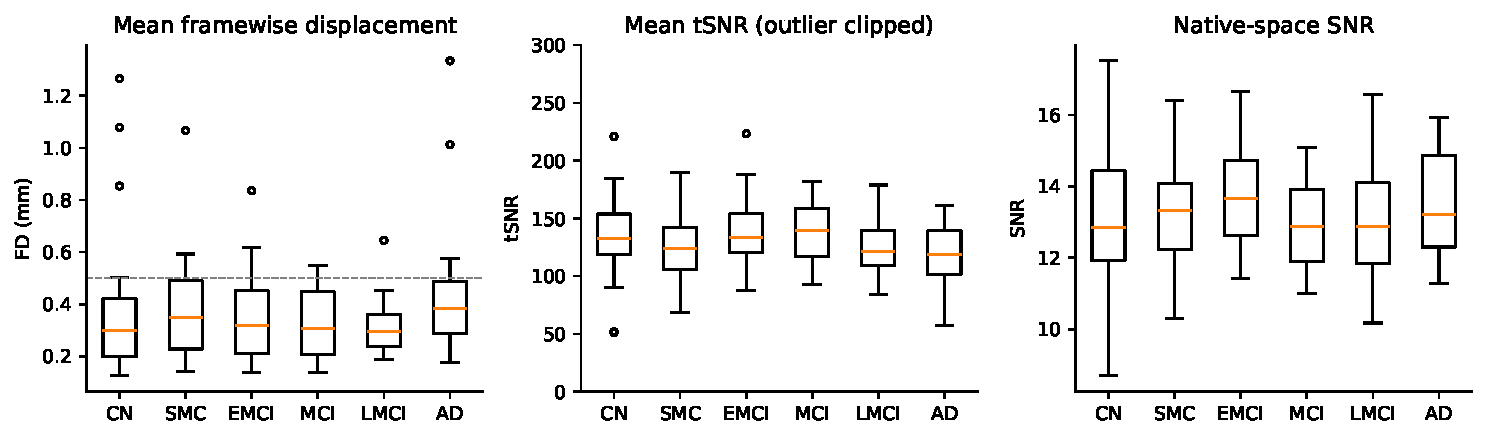
\includegraphics[width=\textwidth]{figures/qc_by_group.pdf}
\caption{Per-acquisition QC by group. Dashed line: 0.5~mm FD reference. The
tSNR axis is clipped at 300 to show the bulk of the distribution.}
\label{fig:qc}
\end{figure}

\paragraph{Discussion.} QC is broadly comparable across groups. Differences
in signal quality are modest and do not follow the stage order (median tSNR
119--139, mean SNR 12.9--13.8). This matters because a quality difference
between classes could be learnt as a spurious ``biomarker''. AD does have
both the lowest median tSNR and the highest motion (mean FD 0.44~mm, 27.7\%
of volumes above 0.5~mm), so both will be checked as confounds. 155 of the 165
acquisitions carry a \textsc{warn} flag, every one of them for FD. Under the frozen
policy these are flagged, not excluded. Because motion is known to bias
connectivity estimates~\cite{power2012,satterthwaite2013}, mean FD will be
used as a covariate and confound check in the modelling stage. All 165
acquisitions are 4-D, on the identical 4~mm grid, with valid masks and no
NaN/Inf. Source checksums were unchanged before and after processing in 165/165.

\begin{figure}[H]
\centering
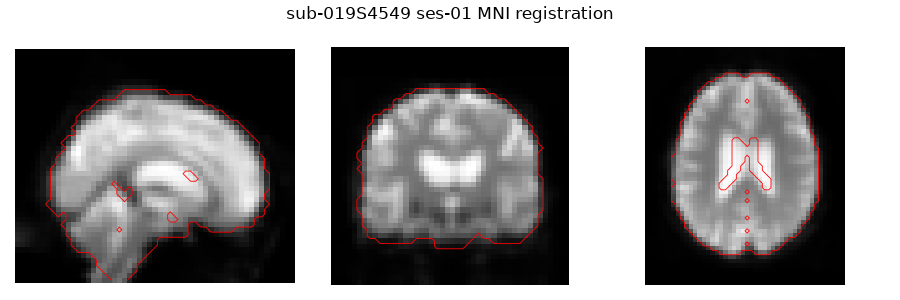
\includegraphics[width=0.9\textwidth]{figures/pilot_registration_qc.png}\\[2pt]
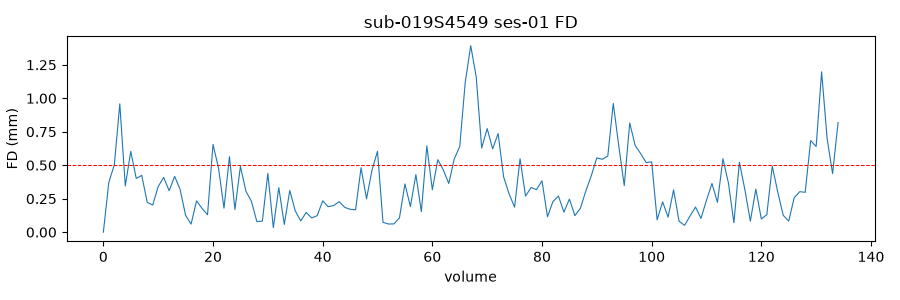
\includegraphics[width=0.9\textwidth]{figures/pilot_fd_plot.png}\\[2pt]
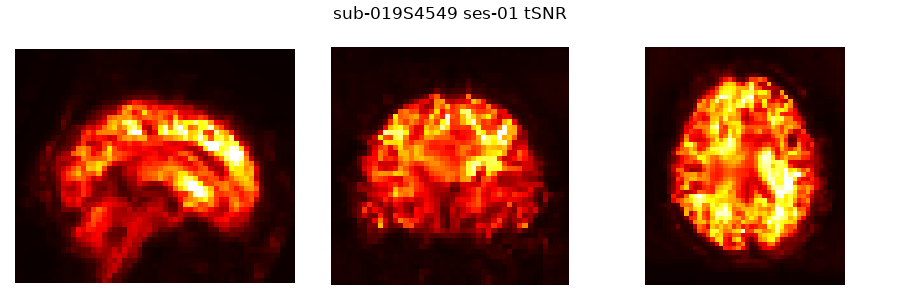
\includegraphics[width=0.9\textwidth]{figures/pilot_tsnr_map.png}
\caption{Pipeline QC output for the pilot acquisition (AD, sub-019S4549,
ses-01): MNI registration overlay (top), framewise displacement (middle) and
tSNR map (bottom).}
\label{fig:pilotqc}
\end{figure}

\section{Parcellation and Biomarker Validation}
Table~\ref{tab:biovalid} gives the dataset-level verification over all 165
acquisitions. The checks re-read the saved files and recompute the derived
quantities independently of the generation code.

\begin{table}[H]
\centering
\caption{Dataset-level biomarker verification (165 acquisitions)}\label{tab:biovalid}
\small
\begin{tabular}{lr}
\toprule
\hdr Check & Result\\
\midrule
Acquisitions with all 246 ROIs present / any zero-voxel ROI & 165/165 \;/\; 0\\
ROI voxel count (min / median / max)                     & 10 / 68 / 186\\
ROI time series shape $(135,246)$                         & 165/165\\
Non-finite values; zero-variance ROIs                     & 0; 0\\
ALFF non-finite or negative values                       & 0\\
ReHo values outside $[0,1]$; observed range              & 0; 0.235--0.823\\
FC max diagonal error / max asymmetry                     & $2.2\times10^{-16}$ / $2.2\times10^{-16}$\\
FC negative off-diagonal share (mean, range)              & 50.1\% (45.6--53.1\%)\\
\textbf{DC recomputed from stored FC, max difference}     & \textbf{0.000}\\
FC strength recomputed, max difference                    & $6.9\times10^{-18}$\\
Acquisitions passing all consistency checks; failures     & \textbf{165/165}; 0\\
\bottomrule
\end{tabular}
\end{table}

The DC result is the strongest evidence here. It shows that the files are well
formed and also that the stored values are exactly what the documented
definition produces, in every acquisition. About half of all off-diagonal
correlations are negative. This is expected after global-signal
regression~\cite{murphy2017}, and it is why DC and FC are kept signed.

\section{Normalisation Results}
Figure~\ref{fig:scaling} shows why within-subject normalisation is needed. Raw
mean ALFF spans more than two orders of magnitude between acquisitions and
mostly reflects intensity scaling, while ReHo stays in a narrow band. After
normalisation, mean mALFF and mean mReHo equal $1.000000$ and std(DC$_z$)
equals $1.000000$ in all 165 acquisitions. Mean DC$_z$ is at most
$1.6\times10^{-16}$. The Fisher-$z$ FC is symmetric (max asymmetry
$5.3\times10^{-15}$), its diagonal is exactly 0 in 165/165 and its range is
$-2.27$ to $2.59$. The $\pm0.999999$ clip was \emph{never} triggered, and no
input or output contains NaN or Inf.

\begin{figure}[H]
\centering
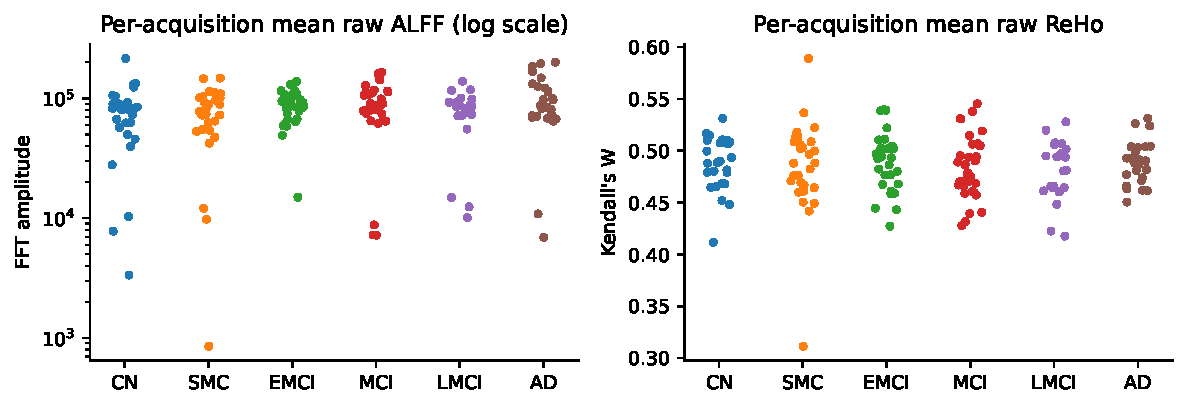
\includegraphics[width=0.95\textwidth]{figures/alff_reho_scaling.pdf}
\caption{Per-acquisition mean raw ALFF (log scale) and raw ReHo by group. ALFF
varies by a factor of about 250 because it scales with raw BOLD intensity.}
\label{fig:scaling}
\end{figure}

\begin{figure}[H]
\centering
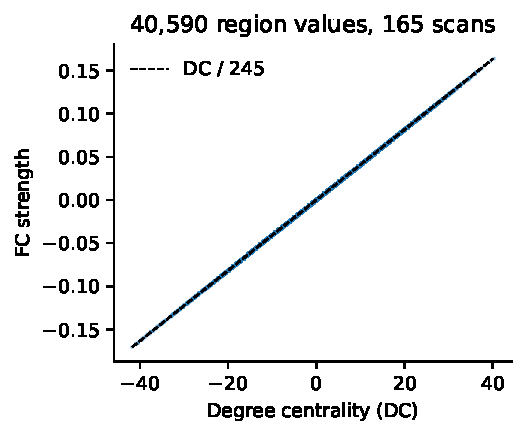
\includegraphics[width=0.45\textwidth]{figures/dc_vs_fcstrength.pdf}
\caption{DC against FC strength for all 40,590 region values. Every point
lies on $\text{FCS}=\text{DC}/245$ ($r=1.0$), so FC strength is excluded as
redundant.}
\label{fig:dcfcs}
\end{figure}

\section{Descriptive Group-Level Connectivity}
Figure~\ref{fig:groupfc} shows the group-mean Fisher-$z$ connectivity, averaged
first within each subject and then across subjects so that multi-session
subjects are not over-weighted. All six groups show the same broad structure:
strong positive coupling within lobes (the diagonal blocks), a distinct
subcortical block, and weak or negative coupling between several lobes. These maps are \emph{descriptive only}. No
statistical test has been run, and group means do not show whether
individuals can be told apart. That question is for the planned model, under
subject-grouped validation.

\begin{figure}[H]
\centering
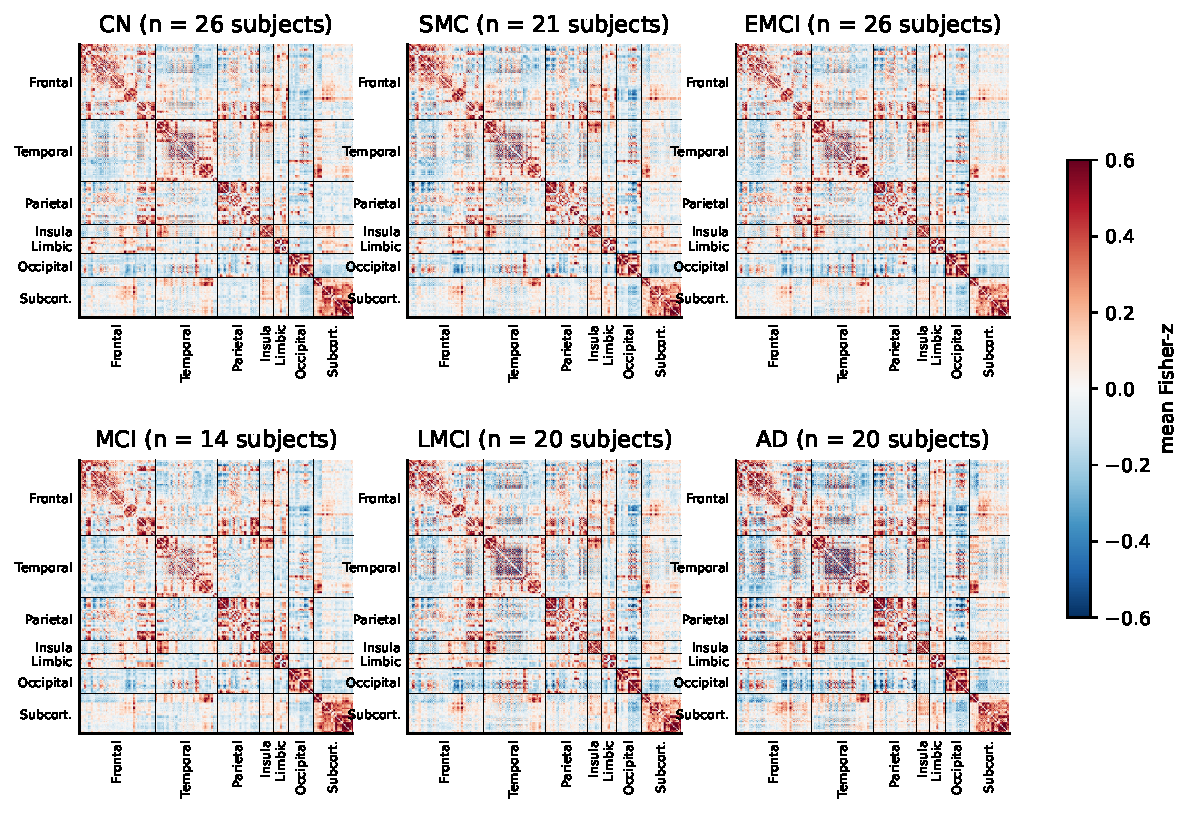
\includegraphics[width=\textwidth]{figures/group_mean_fc.pdf}
\caption{Group-mean Fisher-$z$ functional connectivity on the Brainnetome-246
atlas, ordered by lobe (subject-level averaging).}
\label{fig:groupfc}
\end{figure}

\section{Comparison with Existing Work}
Table~\ref{tab:compare} compares the design choices of this pipeline with
those of conventional T1w-based rs-fMRI pipelines such as
DPABI~\cite{yan2016}. The main differences come from the dataset
constraints. Where a conventional pipeline would rely on missing information,
this project substitutes a documented alternative or records the step as not
performed.

\begin{table}[H]
\centering
\caption{Design comparison with a conventional rs-fMRI pipeline}\label{tab:compare}
\small
\begin{tabularx}{\textwidth}{>{\raggedright\arraybackslash}p{2.9cm}>{\raggedright\arraybackslash}X>{\raggedright\arraybackslash}X}
\toprule
\hdr Aspect & Typical pipeline with T1w and full metadata & This project (BOLD-only ADNI subset)\\
\midrule
Spatial normalisation & BOLD $\rightarrow$ T1w $\rightarrow$ template & direct EPI $\rightarrow$ MNI152 (ANTs SyN)\\
WM/CSF signals & subject-specific tissue segmentation & template priors with a per-acquisition reliability gate\\
Slice timing & corrected from header timing & audited as not recoverable; not performed, not guessed\\
Band-pass vs.\ TR & one fixed band for all scans & band checked against each scan's Nyquist frequency; 8 incompatible scans rejected with logged reason\\
Atlas labels & toolbox-internal resampling & nearest-neighbour only, coverage verified per scan\\
Biomarker verification & toolbox outputs used directly & exact independent recomputation, 165/165\\
Scaling / splitting & whole-dataset statistics and scan-level splits are known leakage sources~\cite{wen2020} & within-subject now; cross-subject only on training folds; subject-grouped CV\\
\bottomrule
\end{tabularx}
\end{table}

Leakage between training and test data, through subject overlap or
whole-dataset preprocessing statistics, is a recurring problem in AD
classification studies and can inflate reported accuracy
substantially~\cite{wen2020}. Small neuroimaging samples also produce wide
error bars~\cite{varoquaux2018}. This project avoids both by design. Every
statistic computed so far is within-acquisition, and the evaluation protocol
is fixed as repeated, stratified, subject-grouped cross-validation before any
model is trained. Accuracy comparisons with published classifiers will be made
in the final review, once the model exists.

\section{Limitations}
\begin{itemize}
  \item No T1w image exists, so registration is EPI-to-template, WM/CSF signals
        come from priors (the CSF prior failed the gate in every
        acquisition), and CNR cannot be computed.
  \item Slice-timing correction was impossible. Undocumented private DICOM tags
        cannot be completely ruled out as carrying such information.
  \item 8 of 173 eligible acquisitions (TR $=6.02$~s) are excluded unless the
        methodology is revisited for that protocol.
  \item Validation so far is mathematical and structural, not biological;
        diagnostic value can only be shown by the model.
  \item The cohort is small (127 subjects, 14 in MCI). The LMCI clinical
        table is missing. Hypertension and diabetes are available only as
        broad medical-history categories.
\end{itemize}

\section{Plan for the Remaining Work}\label{sec:plan}
Figure~\ref{fig:gantt} gives the tentative schedule up to the final review.

% TODO: adjust months to the department's review calendar.
\begin{figure}[H]
\centering
\resizebox{\textwidth}{!}{%
\begin{ganttchart}[
    hgrid, vgrid,
    x unit=0.40cm, y unit chart=0.62cm,
    title height=1,
    title label font=\small,
    bar label font=\small,
    milestone label font=\small\itshape,
    bar/.append style={fill=blue!25},
    bar height=0.55,
    group/.append style={fill=black!60},
    milestone/.append style={fill=red!60}]{1}{24}
  \gantttitle{Oct}{4}\gantttitle{Nov}{4}\gantttitle{Dec}{4}
  \gantttitle{Jan}{4}\gantttitle{Feb}{4}\gantttitle{Mar}{4}\\
  \ganttbar{Comorbidity data cleaning}{1}{4}\\
  \ganttbar{Cohort index, grouped CV folds}{3}{5}\\
  \ganttbar{Train-fold scaling, baselines}{5}{8}\\
  \ganttbar{Multi-attention transformer}{7}{12}\\
  \ganttbar{Meta-learning}{11}{15}\\
  \ganttbar{Comorbidity fusion}{13}{16}\\
  \ganttbar{Bayesian ordinal classifier}{15}{18}\\
  \ganttbar{Uncertainty \& explainability}{18}{20}\\
  \ganttbar{Evaluation, ablations, report}{20}{24}\\
  \ganttmilestone{Final review}{24}
\end{ganttchart}}
\caption{Tentative schedule for the modelling stages (weeks grouped by month)}
\label{fig:gantt}
\end{figure}

\section{Conclusion}
The data foundation is complete. 175 ADNI rs-fMRI acquisitions have been
audited, and 165 have been preprocessed, parcellated, turned into ALFF, ReHo,
FC and DC biomarkers and normalised within subject, with zero processing
failures after preprocessing. Every derived value has been verified
independently. Each limitation of the BOLD-only dataset is handled by a
documented substitution or exclusion rather than by fabrication. The
work also corrected the Review-I design in two places. The regional feature
matrix is $246\times3$, because FC strength is redundant. The unit of
validation is the subject, of which there are 127. The next phase builds the
comorbidity-aware Meta-Bayesian ordinal model on these features and evaluates
it under subject-grouped cross-validation.

% =====================================================================
\begin{thebibliography}{99}

\bibitem{alz2024} Alzheimer's Association, ``2024 Alzheimer's disease facts and figures,'' \textit{Alzheimer's \& Dementia}, vol.~20, no.~5, pp.~3708--3821, 2024. DOI: \url{https://doi.org/10.1002/alz.13809}.

\bibitem{livingston2020} G. Livingston \textit{et al.}, ``Dementia prevention, intervention, and care: 2020 report of the Lancet Commission,'' \textit{The Lancet}, vol.~396, no.~10248, pp.~413--446, 2020. DOI: \url{https://doi.org/10.1016/S0140-6736(20)30367-6}.

\bibitem{jessen2014} F. Jessen \textit{et al.}, ``A conceptual framework for research on subjective cognitive decline in preclinical Alzheimer's disease,'' \textit{Alzheimer's \& Dementia}, vol.~10, no.~6, pp.~844--852, 2014. DOI: \url{https://doi.org/10.1016/j.jalz.2014.01.001}.

\bibitem{petersen2010} R. C. Petersen \textit{et al.}, ``Alzheimer's Disease Neuroimaging Initiative (ADNI): Clinical characterization,'' \textit{Neurology}, vol.~74, no.~3, pp.~201--209, 2010. DOI: \url{https://doi.org/10.1212/WNL.0b013e3181cb3e25}.

\bibitem{biswal1995} B. Biswal, F. Z. Yetkin, V. M. Haughton, and J. S. Hyde, ``Functional connectivity in the motor cortex of resting human brain using echo-planar MRI,'' \textit{Magnetic Resonance in Medicine}, vol.~34, no.~4, pp.~537--541, 1995. DOI: \url{https://doi.org/10.1002/mrm.1910340409}.

\bibitem{greicius2004} M. D. Greicius, G. Srivastava, A. L. Reiss, and V. Menon, ``Default-mode network activity distinguishes Alzheimer's disease from healthy aging: Evidence from functional MRI,'' \textit{Proceedings of the National Academy of Sciences}, vol.~101, no.~13, pp.~4637--4642, 2004. DOI: \url{https://doi.org/10.1073/pnas.0308627101}.

\bibitem{zang2007} Y.-F. Zang \textit{et al.}, ``Altered baseline brain activity in children with ADHD revealed by resting-state functional MRI,'' \textit{Brain and Development}, vol.~29, no.~2, pp.~83--91, 2007. DOI: \url{https://doi.org/10.1016/j.braindev.2006.07.002}.

\bibitem{zang2004} Y. Zang, T. Jiang, Y. Lu, Y. He, and L. Tian, ``Regional homogeneity approach to fMRI data analysis,'' \textit{NeuroImage}, vol.~22, no.~1, pp.~394--400, 2004. DOI: \url{https://doi.org/10.1016/j.neuroimage.2003.12.030}.

\bibitem{zuo2012} X.-N. Zuo \textit{et al.}, ``Network centrality in the human functional connectome,'' \textit{Cerebral Cortex}, vol.~22, no.~8, pp.~1862--1875, 2012. DOI: \url{https://doi.org/10.1093/cercor/bhr269}.


\bibitem{fan2016} L. Fan \textit{et al.}, ``The Human Brainnetome Atlas: A new brain atlas based on connectional architecture,'' \textit{Cerebral Cortex}, vol.~26, no.~8, pp.~3508--3526, 2016. DOI: \url{https://doi.org/10.1093/cercor/bhw157}.

\bibitem{vaswani2017} A. Vaswani \textit{et al.}, ``Attention is all you need,'' in \textit{Advances in Neural Information Processing Systems}, vol.~30, 2017, pp.~5998--6008.

\bibitem{finn2017} C. Finn, P. Abbeel, and S. Levine, ``Model-agnostic meta-learning for fast adaptation of deep networks,'' in \textit{Proc. 34th International Conference on Machine Learning (ICML)}, PMLR vol.~70, 2017, pp.~1126--1135.

\bibitem{mccullagh1980} P. McCullagh, ``Regression models for ordinal data,'' \textit{Journal of the Royal Statistical Society: Series B}, vol.~42, no.~2, pp.~109--142, 1980.

\bibitem{gal2016} Y. Gal and Z. Ghahramani, ``Dropout as a Bayesian approximation: Representing model uncertainty in deep learning,'' in \textit{Proc. 33rd International Conference on Machine Learning (ICML)}, PMLR vol.~48, 2016, pp.~1050--1059.

\bibitem{varoquaux2018} G. Varoquaux, ``Cross-validation failure: Small sample sizes lead to large error bars,'' \textit{NeuroImage}, vol.~180, pp.~68--77, 2018. DOI: \url{https://doi.org/10.1016/j.neuroimage.2017.06.061}.

\bibitem{wen2020} J. Wen \textit{et al.}, ``Convolutional neural networks for classification of Alzheimer's disease: Overview and reproducible evaluation,'' \textit{Medical Image Analysis}, vol.~63, 101694, 2020. DOI: \url{https://doi.org/10.1016/j.media.2020.101694}.

\bibitem{fischl2012} B. Fischl, ``FreeSurfer,'' \textit{NeuroImage}, vol.~62, no.~2, pp.~774--781, 2012. DOI: \url{https://doi.org/10.1016/j.neuroimage.2012.01.021}.

\bibitem{cox1996} R. W. Cox, ``AFNI: Software for analysis and visualization of functional magnetic resonance neuroimages,'' \textit{Computers and Biomedical Research}, vol.~29, no.~3, pp.~162--173, 1996. DOI: \url{https://doi.org/10.1006/cbmr.1996.0014}.

\bibitem{avants2008} B. B. Avants, C. L. Epstein, M. Grossman, and J. C. Gee, ``Symmetric diffeomorphic image registration with cross-correlation: Evaluating automated labeling of elderly and neurodegenerative brain,'' \textit{Medical Image Analysis}, vol.~12, no.~1, pp.~26--41, 2008. DOI: \url{https://doi.org/10.1016/j.media.2007.06.004}.

\bibitem{ciric2022} R. Ciric \textit{et al.}, ``TemplateFlow: FAIR-sharing of multi-scale, multi-species brain models,'' \textit{Nature Methods}, vol.~19, pp.~1568--1571, 2022. DOI: \url{https://doi.org/10.1038/s41592-022-01681-2}.

\bibitem{abraham2014} A. Abraham \textit{et al.}, ``Machine learning for neuroimaging with scikit-learn,'' \textit{Frontiers in Neuroinformatics}, vol.~8, art.~14, 2014. DOI: \url{https://doi.org/10.3389/fninf.2014.00014}.

\bibitem{power2012} J. D. Power, K. A. Barnes, A. Z. Snyder, B. L. Schlaggar, and S. E. Petersen, ``Spurious but systematic correlations in functional connectivity MRI networks arise from subject motion,'' \textit{NeuroImage}, vol.~59, no.~3, pp.~2142--2154, 2012. DOI: \url{https://doi.org/10.1016/j.neuroimage.2011.10.018}.

\bibitem{friston1996} K. J. Friston, S. Williams, R. Howard, R. S. J. Frackowiak, and R. Turner, ``Movement-related effects in fMRI time-series,'' \textit{Magnetic Resonance in Medicine}, vol.~35, no.~3, pp.~346--355, 1996. DOI: \url{https://doi.org/10.1002/mrm.1910350312}.

\bibitem{satterthwaite2013} T. D. Satterthwaite \textit{et al.}, ``An improved framework for confound regression and filtering for control of motion artifact in the preprocessing of resting-state functional connectivity data,'' \textit{NeuroImage}, vol.~64, pp.~240--256, 2013. DOI: \url{https://doi.org/10.1016/j.neuroimage.2012.08.052}.

\bibitem{murphy2017} K. Murphy and M. D. Fox, ``Towards a consensus regarding global signal regression for resting state functional connectivity MRI,'' \textit{NeuroImage}, vol.~154, pp.~169--173, 2017. DOI: \url{https://doi.org/10.1016/j.neuroimage.2016.11.052}.

\bibitem{yan2016} C.-G. Yan, X.-D. Wang, X.-N. Zuo, and Y.-F. Zang, ``DPABI: Data Processing \& Analysis for (Resting-State) Brain Imaging,'' \textit{Neuroinformatics}, vol.~14, no.~3, pp.~339--351, 2016. DOI: \url{https://doi.org/10.1007/s12021-016-9299-4}.

\end{thebibliography}

\end{document}
